\documentclass[11pt,a4paper]{report}
\usepackage[utf8]{inputenc}
\usepackage[T1]{fontenc}
\usepackage[spanish,es-nodecimaldot]{babel}
\usepackage{lmodern,amsmath,amssymb,mathtools}
\usepackage[margin=2.3cm,headheight=15pt]{geometry}
\usepackage{graphicx,xcolor,booktabs,longtable,array,enumitem,fancyhdr}
\usepackage[breakable]{tcolorbox}
\usepackage{hyperref}
\definecolor{plum}{HTML}{5A456A}
\definecolor{lila}{HTML}{EEE7F3}
\hypersetup{colorlinks=true,linkcolor=plum,urlcolor=plum,citecolor=plum,pdftitle={Informe técnico: PINNs e identificabilidad FUCCI},pdfauthor={Bamsi Mendez Posada y Sergio Alejandro Villada Arias}}
\setlength{\parindent}{0pt}
\setlength{\parskip}{4pt}
\setlength{\emergencystretch}{2em}
\makeatletter
\def\@makechapterhead#1{\vspace*{12pt}{\parindent\z@\raggedright\normalfont
\ifnum\c@secnumdepth>\m@ne\large\bfseries\@chapapp\space\thechapter\par\nobreak\vskip12pt\fi
\interlinepenalty\@M\huge\bfseries #1\par\nobreak\vskip24pt}}
\makeatother
\setlist{itemsep=3pt,topsep=4pt}
\pagestyle{fancy}\fancyhf{}
\fancyhead[L]{\small PINNs, inferencia e identificabilidad}
\fancyhead[R]{\small Informe técnico}
\fancyfoot[C]{\thepage}
\newtcolorbox{idea}[1]{breakable,colback=lila,colframe=plum,title={#1},fonttitle=\bfseries,boxrule=.6pt}
\newcommand{\R}{\mathbb R}
\newcommand{\E}{\mathbb E}
\newcommand{\Var}{\operatorname{Var}}
\newcommand{\diag}{\operatorname{diag}}
\newcommand{\RMSE}{\operatorname{RMSE}}
\newcommand{\argmin}{\operatorname*{arg\,min}}

\begin{document}
\begin{titlepage}
\vspace*{1cm}
{\color{plum}\large INFORME TÉCNICO DEL PROYECTO\par}
\vspace{1cm}
{\Huge\bfseries Identificabilidad e incertidumbre en modelos de invasión celular\par}
\vspace{.7cm}
{\LARGE Inferencia clásica y redes neuronales informadas por la física\par}
\vspace{1.1cm}
{\large Bamsi Mendez Posada\\Sergio Alejandro Villada Arias\par}
\vspace{.6cm}
Universidad Nacional de Colombia, Sede Manizales\\
Facultad de Ciencias Exactas y Naturales
\vfill
\begin{idea}{Resumen}
Se estudia la precisión con que datos FUCCI permiten inferir parámetros de un sistema de reacción--difusión. Se comparan una difusividad compartida y dos difusividades libres mediante máxima verosimilitud, perfiles e inferencia con PINNs. La difusión común presenta un intervalo perfilado aproximado del 95\% de $[365.07,1207.68]$ $\mu$m$^2$/h. Al separar las difusiones, sus perfiles no cruzan el umbral dentro de las cotas exploradas y aumenta la dispersión de las estimaciones neuronales. Los resultados distinguen calidad de ajuste, estabilidad del entrenamiento e incertidumbre estadística.
\end{idea}
\vspace{.4cm}
Proyecto presentado en el Segundo Workshop de Estadística, 6 de noviembre de 2026.\\
Edición documental para el repositorio: 8 de noviembre de 2026.
\end{titlepage}
\setcounter{tocdepth}{0}
\tableofcontents
\chapter*{Resumen ejecutivo}
\addcontentsline{toc}{chapter}{Resumen ejecutivo}
El estudio aborda un problema inverso: estimar movimiento y tasas del ciclo celular a partir de densidades observadas en espacio y tiempo. Se emplean 24 posiciones y cuatro tiempos; el tiempo cero determina una condición inicial suavizada, mientras que las 144 densidades posteriores constituyen el objetivo de ajuste.

En el escenario de difusión compartida, el MLE por diferencias finitas es $\widehat D=709.85$ $\mu$m$^2$/h, $\widehat k_r=0.02888$ h$^{-1}$ y $\widehat k_g=0.07162$ h$^{-1}$. Diez resultados finales de PINN tienen media $700.09$ para $D$ y desviación entre entrenamientos $3.04$. Esa desviación mide variabilidad computacional sobre el mismo conjunto observado; no sustituye el intervalo de confianza perfilado.

La extensión a dos difusiones apenas reduce el objetivo estandarizado: de $7.96798$ a $7.95705$. Los perfiles de ambas difusiones carecen de cruces con el umbral del 95\% dentro de $[1,2000]$. Cuatro de diez estimaciones neuronales quedan fuera de las cotas de difusión del MLE, por lo que la comparación requiere reconocer restricciones distintas.

Este informe desarrolla el fundamento matemático, la implementación, los resultados, sus limitaciones y la ruta de reproducción. Las tablas publicadas son evidencia archivada del trabajo presentado; los comandos del repositorio permiten generar nuevos análisis separados. No se atribuyen a este proyecto resultados de cobertura, validación predictiva externa o identificabilidad estructural que no se hayan calculado.
\chapter{Planteamiento y objetivos}
\section{Problema científico}
Un cultivo celular invade una región inicialmente poco ocupada. El avance visible mezcla dos mecanismos: las células se desplazan y también se reproducen. Además, cambian de fase del ciclo celular. Observar que aumenta la densidad en una zona no permite atribuir automáticamente ese aumento a uno solo de esos mecanismos.

FUCCI permite distinguir dos grupos mediante fluorescencia: rojo para G1 y verde para S/G2/M. En vez de observar únicamente la densidad total, disponemos de dos campos. El modelo traduce movimiento, transición y división en ecuaciones. La inferencia intenta recorrer el camino inverso: a partir de las densidades medidas, estimar los parámetros que gobiernan las ecuaciones.

\begin{idea}{Pregunta de investigación}
¿Con qué precisión permiten los datos FUCCI estimar los parámetros de un modelo de invasión celular y cómo cambia su identificabilidad al considerar una difusión compartida o dos difusiones distintas?
\end{idea}

La PINN es una herramienta para resolver ese problema inverso. El objetivo estadístico consiste en averiguar qué tan informativas son las observaciones sobre los parámetros, no únicamente en construir una curva visualmente convincente.

\section{Los dos escenarios}
\begin{center}
\begin{tabular}{lll}\toprule
Escenario & Restricción & Parámetros físicos\\\midrule
1 & $D_r=D_g=D$ & $(D,k_r,k_g)$\\
2 & Difusiones libres & $(D_r,D_g,k_r,k_g)$\\\bottomrule
\end{tabular}
\end{center}
El escenario 1 está contenido en el 2. Imponer difusión común reduce la dimensión de la búsqueda y descarta combinaciones en las que una población difunde mucho y la otra poco. Esta restricción puede aumentar la precisión, pero también podría introducir sesgo si la igualdad fuera inadecuada. El estudio evalúa qué permite sostener este conjunto de datos; no demuestra que ambas poblaciones tengan necesariamente la misma movilidad biológica.

\section{Tres preguntas diferentes}
\begin{enumerate}
\item \textbf{Ajuste:} ¿las densidades predichas se parecen a las observadas? Se examinan curvas, residuos y RMSE.
\item \textbf{Estabilidad computacional:} ¿las distintas inicializaciones llevan a resultados similares? Se examinan diez resultados finales por escenario y los reinicios.
\item \textbf{Precisión estadística:} ¿qué valores paramétricos siguen siendo compatibles con los datos? Se examinan perfiles e intervalos bajo el modelo de observación.
\end{enumerate}
Un algoritmo puede converger siempre al mismo punto en un valle muy ancho de la función objetivo. La repetibilidad del punto elegido no vuelve estrecho el valle. También puede suceder lo contrario: un parámetro bien informado por los datos puede resultar difícil de estimar con un algoritmo mal ajustado.

\section{Aportes y antecedentes}
El modelo, los datos experimentales y el contraste entre una y dos difusiones tienen antecedentes en Simpson y colaboradores \cite{simpson}. El aporte del proyecto es estudiar la PINN inversa sobre este problema, contrastarla con un ajuste clásico coherente, repetir entrenamientos y verificar sus parámetros con un solucionador independiente de la red. Los perfiles proporcionan el contexto estadístico para interpretar esa comparación.

No se recolectaron nuevos experimentos biológicos. No se implementó una PINN bayesiana en los resultados del póster. Tampoco se demostró una ventaja general de velocidad o precisión frente a los métodos clásicos. La contribución defendible es metodológica y aplicada: conectar el comportamiento del entrenamiento con la información que realmente contienen las observaciones.



\chapter{Experimento, datos y significado biológico}
\section{Qué significa FUCCI}
FUCCI corresponde a \emph{Fluorescent Ubiquitination-based Cell Cycle Indicator}. El sistema de marcadores permite relacionar fluorescencia y fase del ciclo. En el modelo reducido se agrupan las células en G1, representadas por $r$, y S/G2/M, representadas por $g$. Los colores indican estados de una misma población celular; no son dos especies independientes.

G1 precede a la síntesis de ADN; S corresponde a esa síntesis, G2 a la preparación posterior y M a la división. El modelo agrupa S/G2/M para mantener un número manejable de estados. Las tasas efectivas resumen procesos biológicos que, a escala individual, son más complejos que dos transiciones exponenciales.

\section{Unidad de observación y tamaño de la información}
\begin{center}
\begin{tabular}{lr}\toprule
Característica & Valor\\\midrule
Posiciones & 24\\
Dominio espacial & $0$ a $1242\,\mu\mathrm m$\\
Separación entre posiciones & $54\,\mu\mathrm m$\\
Tiempos & $0,16,32,48$ h\\
Puntos espacio-temporales & $24\times4=96$\\
Densidades por punto & 2\\
Valores de densidad disponibles & 192\\
Valores iniciales & 48\\
Valores incluidos en el ajuste & 144\\\bottomrule
\end{tabular}
\end{center}
En cada posición y tiempo se registra una densidad roja y una verde. La tabla original conserva también conteos, pero la inferencia presentada utiliza densidades adimensionales y errores gaussianos. No utiliza una verosimilitud de Poisson para los conteos.

Los 144 valores no deben describirse como 144 experimentos biológicos independientes. Son mediciones espaciales y temporales de un sistema. La independencia entra como supuesto del modelo de error y merece revisión; no se deduce del número de filas de una tabla.

\section{Por qué se excluye el tiempo inicial del objetivo}
Las observaciones en $t=0$ se emplean para construir los perfiles iniciales. Después se ajusta la evolución en 16, 32 y 48 horas. Así, el objetivo principal no vuelve a contar el tiempo inicial como un conjunto de residuos ordinarios independientes de una condición inicial que ya se construyó con esos mismos datos.

Esto no elimina el error de medición inicial: simplemente se condiciona la inferencia a una función inicial fija. Para propagar esa incertidumbre habría que introducir coeficientes iniciales como parámetros auxiliares, o simular y reajustar el procedimiento completo.

\section{Suavizado inicial con cosenos}
La implementación que sustenta los resultados usa
\begin{equation}
r_0(x)=\sum_{j=0}^{8}a_j\cos(j\pi x/L),\qquad
g_0(x)=\sum_{j=0}^{8}b_j\cos(j\pi x/L),\quad L=1242.
\end{equation}
Hay nueve coeficientes por población, incluido el término constante. Se estiman por mínimos cuadrados con los 24 valores iniciales. Si $A_{ij}=\cos(j\pi x_i/L)$, se resuelve $\min_a\|Aa-y_0^{(r)}\|^2$ y análogamente para $b$.

Cada coseno tiene derivada nula en los extremos. Por tanto, el perfil suavizado es compatible con flujo nulo. La igualdad exacta con $r_0$ no significa que la red pase exactamente por las 24 observaciones: estas se aproximaron antes mediante la expansión truncada.

El número de modos controla flexibilidad. Pocos modos borran detalles; demasiados pueden seguir ruido y crear oscilaciones. Una serie de cosenos sin restricciones tampoco garantiza por sí sola densidades no negativas.



\chapter{Derivación y lectura del modelo de reacción--difusión}
\section{Sistema y unidades}
\begin{align}
\partial_t r&=D_r\partial_{xx}r-k_rr+2k_gg(1-r-g),\label{eq:r}\\
\partial_t g&=D_g\partial_{xx}g+k_rr-k_gg(1-r-g).\label{eq:g}
\end{align}
Las densidades son adimensionales, $x$ se mide en micrómetros y $t$ en horas. Así, $D_r,D_g$ tienen unidades $\mu\mathrm m^2/\mathrm h$ y $k_r,k_g$ tienen unidades $\mathrm h^{-1}$. Cada término del lado derecho debe tener unidades de densidad por hora.

\section{Difusión: por qué aparece una segunda derivada}
Sea $J_r=-D_r\partial_x r$ el flujo de células rojas. La ley de balance local es $\partial_t r=-\partial_xJ_r+$ fuentes. Con difusividad constante, $-\partial_xJ_r=D_r\partial_{xx}r$.

En un máximo local suave, $r_{xx}<0$, de modo que la difusión reduce la densidad; en un mínimo, $r_{xx}>0$ y la aumenta. La difusión suaviza diferencias espaciales. Una pendiente constante produce flujo, pero no acumulación local si entra tanto como sale: la acumulación depende de la variación del flujo, de ahí la segunda derivada.

$D$ no es una velocidad. Para difusión ideal unidimensional sin fronteras, la escala de desplazamiento cuadrático es $\sqrt{2Dt}$. Con $D\approx710$ y $t=16$ h da unos $151\,\mu\mathrm m$. Es una escala orientativa, no la distancia recorrida por cada célula ni la posición exacta del frente de invasión, que también depende de las reacciones y de las fronteras.

\section{Transición y división: los signos y el factor dos}
El término $k_rr$ representa el paso de rojo a verde. Una transición resta una célula roja y añade una verde; por eso aparece con signos opuestos y no cambia el total.

La división retira una célula verde y produce dos rojas. Su intensidad es $k_gg(1-r-g)$. La ecuación verde tiene un signo negativo y la roja recibe dos veces esa cantidad. El balance neto de una división es una célula adicional.

El factor $1-r-g$ representa disponibilidad de espacio. Si la ocupación total es pequeña, está próximo a uno. Cuando se aproxima a uno, la proliferación se frena. La interpretación biológica presupone densidades en un rango admisible; si una aproximación neuronal produce $r+g>1$, no basta invocar la fórmula para justificar ese resultado.

\section{Balance de la densidad total}
Definiendo $n=r+g$,
\begin{equation}
n_t=D_rr_{xx}+D_gg_{xx}+k_gg(1-n).
\end{equation}
Si $D_r=D_g=D$, queda
\begin{equation}
n_t=Dn_{xx}+k_gg(1-n).\label{eq:total}
\end{equation}
No es una ecuación logística cerrada para $n$: aparece $g$, cuya proporción cambia con el ciclo. Para reemplazar $g$ por una fracción fija de $n$ se necesitaría una aproximación adicional que el póster no adopta.

Con fronteras de flujo nulo,
\begin{equation}
\frac{d}{dt}\int_0^L(r+g)\,dx=\int_0^L k_gg(1-r-g)\,dx.
\end{equation}
La difusión redistribuye células y no crea masa total. Las transiciones tampoco alteran el total. La proliferación sí. Esta identidad es útil tanto para explicar el modelo como para detectar errores de signos en una implementación.

\section{Condiciones de frontera e iniciales}
Se imponen
\[
r_x(0,t)=r_x(L,t)=g_x(0,t)=g_x(L,t)=0,
\qquad r(x,0)=r_0(x),\quad g(x,0)=g_0(x).
\]
Flujo nulo significa ausencia de intercambio a través de los bordes del dominio modelado; no significa densidad cero ni ausencia de movimiento dentro del cultivo. Es una hipótesis de cierre de la ventana espacial. Si el experimento intercambiara células de forma importante a través de esos bordes, habría que revisar el modelo.

\section{Escalas temporales y adimensionalización}
Con tasas cercanas a $k_r=0.02888$ y $k_g=0.07162$, las escalas inversas son $1/k_r\approx34.6$ h y $1/k_g\approx14.0$ h. Son escalas nominales: la salida verde está modulada por la densidad y el tiempo de ciclo individual no se estima directamente con esta simple suma.

Definamos $\xi=x/L$ y $\tau=t/T$, con $T=48$ h. Aplicando la regla de la cadena,
\[
\partial_t=T^{-1}\partial_\tau,\qquad
\partial_{xx}=L^{-2}\partial_{\xi\xi}.
\]
La ecuación roja se transforma en
\begin{equation}
r_\tau=\frac{D_rT}{L^2}r_{\xi\xi}-Tk_rr+2Tk_gg(1-r-g).
\end{equation}
Para la difusión común estimada, $DT/L^2\approx0.0221$, $Tk_r\approx1.386$ y $Tk_g\approx3.438$. Cambiar coordenadas sin transformar estos coeficientes modifica el problema físico y puede producir parámetros erróneos aunque disminuya la pérdida.



\chapter{Inferencia clásica y solución numérica}
\section{Qué se conoce y qué se busca}
En el problema directo, los parámetros y las condiciones iniciales son conocidos y buscamos $r(x,t),g(x,t)$. En el inverso, observamos parte de esos campos y buscamos los parámetros. Denotemos por $\mathcal G(\theta)$ la aplicación que resuelve la EDP y evalúa sus soluciones en los puntos observados. El problema inverso compara $y$ con $\mathcal G(\theta)$.

La dificultad no depende solamente del número de datos. Si dos vectores paramétricos producen prácticamente el mismo $\mathcal G(\theta)$, observaciones ruidosas tendrán poca capacidad para distinguirlos.

\section{Modelo de observación y verosimilitud}
Para $m=1,\ldots,n$, $n=144$, se supone
\begin{equation}
Y_m=\mathcal G_m(\theta)+\varepsilon_m,\qquad
\varepsilon_m\overset{\mathrm{iid}}\sim N(0,\sigma^2),\quad \sigma=0.05.
\end{equation}
La densidad conjunta de los datos, vista como función de $\theta$, es
\[
L(\theta;y)=(2\pi\sigma^2)^{-n/2}
\exp\left[-\frac{1}{2\sigma^2}\sum_{m=1}^n(y_m-\mathcal G_m(\theta))^2\right].
\]
Tomando logaritmos,
\begin{align}
\ell(\theta)&=-\frac n2\log(2\pi\sigma^2)-\frac12Q(\theta),\\
Q(\theta)&=\sum_{m=1}^{144}\left(\frac{y_m-\mathcal G_m(\theta)}{0.05}\right)^2.
\end{align}
Como el primer término es constante respecto de $\theta$, maximizar $\ell$ equivale a minimizar $Q$. Esta es la justificación de llamar MLE al ajuste de mínimos cuadrados bajo estos supuestos. Una pérdida cuadrática arbitraria no recibe automáticamente esa interpretación.

\section{RMSE y objetivo ponderado}
\begin{equation}
\RMSE=\sqrt{\frac1n\sum e_m^2}=\sigma\sqrt{Q/n}.
\end{equation}
En el escenario 1, $Q=7.967975$ y $\RMSE=0.0117615$. El objetivo suma errores estandarizados; el RMSE se expresa en unidades de densidad y promedia los 144 errores.

Los archivos llaman \texttt{chi2} a $Q$. Ese nombre no demuestra que el valor observado siga exactamente una distribución chi-cuadrado ni que ya se haya efectuado una prueba de bondad de ajuste.

\section{Supuestos que determinan la interpretación}
\begin{itemize}
\item \textbf{Normalidad:} los errores aditivos se modelan como gaussianos, aunque las densidades sean acotadas.
\item \textbf{Independencia:} se ignoran correlaciones entre posiciones, tiempos y colores.
\item \textbf{Homocedasticidad:} todos los residuos usan la misma desviación estándar.
\item \textbf{Escala fijada:} $0.05$ es un supuesto de referencia, no una desviación estimada por las diez corridas.
\item \textbf{Condición inicial fija:} los intervalos no incluyen su incertidumbre.
\item \textbf{Modelo dinámico adoptado:} no se separa automáticamente error experimental de discrepancia del modelo biológico.
\end{itemize}
Si se cambiara solamente una $\sigma$ común y fija, el mínimo clásico de $Q$ quedaría en el mismo punto, pero los perfiles cambiarían de escala y los intervalos cambiarían de ancho. Con pesos distintos para colores o tiempos podría cambiar también el estimador.

\section{Discretización e integración temporal}
El método de líneas discretiza el espacio y conserva el tiempo como variable continua. En un nodo interior,
\[
r_{xx}(x_i,t)\approx\frac{r_{i-1}(t)-2r_i(t)+r_{i+1}(t)}{h^2}.
\]
La aproximación tiene error espacial de orden $h^2$ para soluciones suficientemente suaves. En la implementación de referencia se emplean 139 nodos, por lo que $h=1242/138=9\,\mu\mathrm m$. Las posiciones observadas, separadas $54\,\mu\mathrm m$, coinciden con uno de cada seis nodos de esta malla.

En la frontera izquierda, un nodo fantasma reflejado satisface $r_{-1}=r_1$ y produce $r_{xx}(0,t)\approx2(r_1-r_0)/h^2$. El mismo principio se aplica al extremo derecho y a $g$.

El sistema resultante tiene $278$ variables dinámicas. Se integra con BDF, tolerancia relativa $10^{-7}$, absoluta $10^{-9}$ y Jacobiano analítico. BDF es un método implícito adecuado para sistemas rígidos, como los que aparecen al discretizar difusión. Las tolerancias controlan el integrador; no prueban por sí solas que el error espacial sea despreciable.

\section{Optimización y restricciones}
El ajuste utiliza mínimos cuadrados no lineales con cotas
\[
1\le D,D_r,D_g\le2000,\qquad 10^{-4}\le k_r,k_g\le0.2.
\]
Las difusiones se escalan por $1000$ y las tasas por $0.05$ para reducir desequilibrios de magnitud. Se verificaron varios inicios: tres para el escenario 1 y cuatro para el escenario 2. La coincidencia de los objetivos es evidencia de robustez frente a esos inicios, no una demostración del mínimo global.

Una comparación justa requiere igualar datos, estado inicial, fronteras, parámetros, evaluación y restricciones. En este proyecto las cotas paramétricas de la PINN y del MLE no son idénticas; se informa explícitamente esa diferencia.

\chapter{Inferencia mediante redes informadas por la física}
\section{Idea básica y problema de optimización}
Una red neuronal aproxima los campos de densidad. Sus pesos $w$ determinan la forma de los campos y los parámetros físicos $\theta$ determinan la ecuación que esos campos deben satisfacer. Se optimizan ambos:
\[
\min_{w,\theta}\;\mathcal L_{\rm datos}(w)+\lambda\mathcal L_{\rm EDP}(w,\theta).
\]
La primera pérdida favorece cercanía a las observaciones. La segunda penaliza que la función neuronal incumpla la ecuación. Los parámetros físicos no son todos los pesos de la red: hay tres o cuatro parámetros de interés y muchos pesos auxiliares que representan las funciones.

\section{Arquitectura de la implementación}
La implementación \texttt{pinn.py} del paquete que sustenta las tablas usa por defecto cuatro capas ocultas de 32 neuronas, activación $\tanh$, dos salidas, inicialización Xavier y precisión de 64 bits. Recibe
\[
z=(\cos(\pi\xi),\cos(2\pi\xi),\cos(3\pi\xi),2\tau-1).
\]
Las funciones de salida se construyen como
\begin{equation}
r_w(\xi,\tau)=r_0(\xi)+0.1\tau N_r(z;w),\qquad
g_w(\xi,\tau)=g_0(\xi)+0.1\tau N_g(z;w).
\label{eq:hard}
\end{equation}
Estos son detalles del código revisado, no todos aparecen impresos en el póster. Los valores por defecto describen la implementación disponible; un registro específico de ejecución prevalecería si documentara cambios de configuración.

\section{Por qué se satisfacen exactamente las condiciones}
Cuando $\tau=0$, el término corrector desaparece, luego $r_w=r_0$ y $g_w=g_0$. Para la frontera, aplicando la regla de la cadena,
\[
\partial_\xi N_r(z)=\sum_{j=1}^{3}\frac{\partial N_r}{\partial z_j}
[-j\pi\sin(j\pi\xi)].
\]
En $\xi=0,1$ todos los senos son cero, y la derivada de la condición inicial también lo es. Así se impone flujo nulo sin términos de penalización separados.

Esta construcción es una restricción fuerte de condiciones iniciales y de frontera. La EDP sigue siendo una restricción blanda, satisfecha aproximadamente mediante la pérdida. Además, la fórmula \eqref{eq:hard} no impone $r,g\ge0$ ni $r+g\le1$; esas propiedades deben comprobarse en los campos.

\section{Diferenciación automática}
La red es una composición de operaciones diferenciables. La diferenciación automática aplica la regla de la cadena sobre ese cálculo para obtener derivadas respecto de $\xi$, $\tau$ y los pesos. Para $r_{\xi\xi}$ se diferencia nuevamente $r_\xi$.

No se están diferenciando directamente los datos ruidosos. Tampoco se trata de diferencias finitas entre evaluaciones cercanas ni de producir una fórmula simbólica cerrada. Se deriva la función implementada por la red, con los límites de precisión numérica correspondientes. Derivar correctamente una red no garantiza que esa red represente correctamente la solución física.

$\tanh$ es suave, lo que permite derivadas segundas ordinarias. Una red ReLU convencional es lineal por tramos y tiene segunda derivada nula casi en todas partes; por eso no es una sustitución directa apropiada para este residuo fuerte de segundo orden.

\section{Residuos diferenciales y función de pérdida}
En coordenadas adimensionales,
\begin{align}
f_r&=r_\tau-\frac{D_rT}{L^2}r_{\xi\xi}+Tk_rr-2Tk_gg(1-r-g),\\
f_g&=g_\tau-\frac{D_gT}{L^2}g_{\xi\xi}-Tk_rr+Tk_gg(1-r-g).
\end{align}
El código promedia la suma de los errores de ambos colores sobre $72$ pares posición--tiempo:
\[
\mathcal L_{\rm datos}=\frac{1}{72\sigma^2}\sum_{i=1}^{72}
\{(r_w-y_i^{(r)})^2+(g_w-y_i^{(g)})^2\}=Q_{\rm red}/72.
\]
La pérdida diferencial es
\[
\mathcal L_{\rm EDP}=\frac1{N_f}\sum_{j=1}^{N_f}(f_r(z_j)^2+f_g(z_j)^2).
\]
Importa el factor 72: promediar sobre 144 componentes cambiaría la pérdida de datos por un factor dos y, manteniendo $\lambda$, cambiaría el equilibrio de penalización.

Los puntos de colocación $z_j$ no son nuevas mediciones biológicas. Son ubicaciones donde se evalúa la ecuación. Añadirlos puede mejorar la aproximación numérica, pero no crea información experimental independiente.

\section{Positividad, escalas y entrenamiento}
Los parámetros se representan como $\theta_j=s_j\exp(\eta_j)$, con $s_j=1000$ para difusiones y $s_j=0.05$ para tasas. Esto garantiza positividad, pero no las cotas $[1,2000]$ usadas por el ajuste clásico. Tampoco equivale a colocar una distribución previa sobre los parámetros.

La rutina disponible combina Adam y refinamiento L-BFGS. Por defecto usa 8000 pasos Adam, un presupuesto de 2500 iteraciones L-BFGS, 1500 puntos de colocación y un peso diferencial que aumenta de $10$ a $2000$ durante el primer 60\% de Adam. Remuestrea colocación cada 100 pasos, refuerza tiempos tempranos y utiliza cinco bloques L-BFGS con colocación renovada. La evaluación diferencial final usa puntos nuevos. No hay que confundir un presupuesto de iteraciones con el número efectivo de evaluaciones de función de L-BFGS.

Adam permite avanzar en el problema conjunto; L-BFGS aproxima información de curvatura para refinar. La continuación del peso evita exigir desde el inicio el mismo compromiso final entre ajuste y ecuación. No existe garantía general de convergencia global para este problema no convexo.

\section{Reinicios y criterio de aceptación}
El controlador disponible usa un umbral $\mathcal L_{\rm EDP,val}\le10^{-5}$, permite hasta tres intentos y modifica las inicializaciones. Selecciona un intento válido o, si no existe, el de menor residuo. Este criterio no usa el verdadero parámetro ni el MLE.

El póster reporta diez resultados finales por escenario y señala que dos corridas del escenario 1 requirieron reinicio. Por ello, ``poca dispersión final'' describe el procedimiento con reinicios. No significa que todos los primeros intentos hayan tenido éxito ni que el entrenamiento sea infalible.



\chapter{Identificabilidad: de la intuición a los perfiles}
\section{Identificabilidad estructural y práctica}
La identificabilidad estructural pregunta si, con observaciones ideales y un esquema de observación especificado, parámetros distintos pueden producir exactamente la misma distribución de observaciones. En el modelo gaussiano de varianza fija, se relaciona con la inyectividad de la aplicación de parámetros a las predicciones observables.

La identificabilidad práctica pregunta si el experimento disponible permite distinguir parámetros con una precisión útil, considerando ruido, cantidad y distribución de observaciones. Un problema puede ser estructuralmente identificable y prácticamente muy débil. En nuestro trabajo no se presentó una demostración formal de identificabilidad estructural.

\section{Ejemplo de confusión paramétrica}
Como ejemplo didáctico, ajeno a los resultados FUCCI, consideremos
\[
u_t=Du_{xx}-ku,\quad u(x,0)=A\cos(qx),
\]
con $q=j\pi/L$ y fronteras de Neumann. Su solución es
\[
u(x,t)=A\cos(qx)e^{-(Dq^2+k)t}.
\]
Los datos de este único modo identifican la combinación $Dq^2+k$. Si aumentamos $D$ y reducimos $k$ en la cantidad correspondiente, la solución permanece igual. Ningún optimizador puede recuperar información que ese experimento no distingue.

Con dos modos distintos, $q_1\ne q_2$, y tasas de decaimiento $a_1,a_2$, se obtiene
\[
D=\frac{a_2-a_1}{q_2^2-q_1^2},\qquad k=a_1-Dq_1^2.
\]
Este ejemplo explica por qué un diseño más informativo puede resolver una confusión. No demuestra que FUCCI tenga esa degeneración exacta; es una analogía matemática para entender el problema inverso.

\section{Qué hace un perfil de verosimilitud}
Separemos $\theta=(\psi,\lambda)$, donde $\psi$ es el parámetro de interés y $\lambda$ reúne los demás. El perfil es
\[
\ell_p(\psi)=\max_\lambda\ell(\psi,\lambda),\qquad
Q_p(\psi)=\min_\lambda Q(\psi,\lambda).
\]
Para cada valor candidato de $D$, se fija $D$ y se reajustan las tasas. Para un perfil de $D_r$ en el escenario 2 se reajustan $D_g,k_r,k_g$. La pregunta es: ``si este fuera el valor del parámetro, ¿qué tan bien podría explicar los datos el mejor resto del modelo?''

Mantener los otros parámetros fijos en su MLE produce una sección, no un perfil. Puesto que el perfil permite reajustar,
\[
Q_p(\psi)\le Q(\psi,\widehat\lambda).
\]
La sección puede sugerir una precisión excesiva al prohibir compensaciones que sí están disponibles en la inferencia real.

\section{Por qué el umbral es 3.84}
El estadístico de razón de verosimilitudes es
\begin{equation}
W(\psi)=2[\ell(\widehat\theta)-\ell_p(\psi)]
=Q_p(\psi)-Q(\widehat\theta).
\end{equation}
Bajo regularidad y una aproximación asintótica, $W(\psi_0)$ se compara con $\chi_1^2$. El conjunto aproximado de confianza al 95\% es
\begin{equation}
\mathcal C_{.95}=\{\psi:W(\psi)\le3.84146\}.
\end{equation}
Hay un grado de libertad porque fijamos un parámetro de interés, no porque el modelo tenga un solo parámetro. Si se perfilaran conjuntamente dos parámetros, el umbral usual sería otro.

La razón de verosimilitudes sin logaritmo es $\exp[-W(\psi)/2]$. El umbral $3.84146$ corresponde a una razón cercana a $0.1465$. Esto explica por qué otras publicaciones muestran perfiles con un máximo en uno y un umbral cercano a $0.15$, mientras el póster presenta curvas con mínimo en cero.

\section{Leer cruces y ausencia de cruces correctamente}
Dos cruces delimitan un intervalo en la región examinada. Un perfil ancho significa que valores separados deterioran poco la verosimilitud. Si no hay cruce antes de llegar a una cota de búsqueda, no conocemos un extremo estadístico más allá de esa cota.

En el escenario 2 los perfiles de $D_r$ y $D_g$ no cruzan el umbral en $[1,2000]$. Es correcto decir ``no se delimitan intervalos dentro del rango explorado''. No es correcto convertir automáticamente $[1,2000]$ en un IC con extremos determinados por los datos, afirmar que el intervalo es todo $\R$ o concluir no identificabilidad estructural.

Además, las proyecciones univariadas no forman una caja conjunta: que dos valores pertenezcan por separado a sus conjuntos perfilados no asegura que su combinación concreta ajuste bien simultáneamente.

\section{Qué significa un intervalo de confianza del 95\%}
En interpretación frecuentista, el procedimiento produciría intervalos que contienen el parámetro verdadero aproximadamente el 95\% de las veces bajo muestreo repetido y los supuestos pertinentes. Después de observar los datos, el parámetro se considera fijo. El IC no asigna directamente probabilidad posterior al parámetro.

En este estudio no se verificó cobertura mediante simulaciones. La palabra ``aproximado'' importa por el tamaño de la muestra, la no linealidad, las restricciones y la debilidad de ciertas direcciones. La independencia y la escala del error también afectan la calibración.



\chapter{Sensibilidades, Fisher y fuentes de incertidumbre}
\section{Linealizar la respuesta del modelo}
Alrededor de un punto $\theta_0$,
\[
\mathcal G(\theta_0+\delta)\approx\mathcal G(\theta_0)+S\delta,
\qquad S_{mj}=\frac{\partial\mathcal G_m}{\partial\theta_j}.
\]
Una columna de $S$ describe cómo cambian las observaciones predichas al variar un parámetro. Columnas pequeñas indican escasa sensibilidad. Columnas casi proporcionales indican que distintos parámetros producen cambios similares y pueden compensarse.

Para errores gaussianos de varianza conocida,
\[
\mathcal I(\theta)=\sigma^{-2}S^TS.
\]
Si $J$ ya es el Jacobiano de residuos divididos por $\sigma$, entonces $\mathcal I=J^TJ$: no se divide otra vez por $\sigma^2$.

La aproximación $\operatorname{Cov}(\widehat\theta)\approx\mathcal I^{-1}$ es local. La Hessiana exacta del objetivo incluye términos de segundas derivadas multiplicados por residuos; $J^TJ$ es la aproximación Gauss--Newton y coincide con la estructura de la información esperada en el modelo gaussiano correspondiente.

\section{Autovalores, escalado y log-parámetros}
Si $v$ es una dirección paramétrica y $\|Sv\|$ es pequeño, desplazarse en esa dirección modifica poco las predicciones. Un autovalor pequeño de Fisher revela una dirección de baja información local.

El condicionamiento depende de las unidades. Comparar difusiones del orden de cientos con tasas del orden de centésimas sin escalar puede confundir magnitudes con información. En log-parámetros $\eta_j=\log\theta_j$,
\[
\frac{\partial\mathcal G}{\partial\eta_j}=\theta_j\frac{\partial\mathcal G}{\partial\theta_j}.
\]
Las tablas de Fisher de respaldo se interpretan en esta parametrización relativa. Sus autovalores, recalculados aquí, son aproximadamente
\[
\begin{array}{c|l|r}
&\text{autovalores}&\text{condición}\\\hline
\text{Escenario 1}&11.32,\;28.40,\;70.73&6.25\\
\text{Escenario 2}&0.1405,\;5.85,\;27.86,\;71.16&506.42
\end{array}
\]
Son diagnósticos adicionales de las tablas existentes, no cifras impresas en el póster. La correlación local estimada entre las dos difusiones es aproximadamente $-0.951$. Esto es compatible con compensación paramétrica; no significa que las dos poblaciones celulares tengan una correlación biológica negativa de ese valor.

\section{Por qué los perfiles son más informativos que un único error estándar}
La aproximación cuadrática describe una vecindad del óptimo y produce elipsoides. No representa bien asimetrías, límites, valles curvos o varios mínimos. En las tablas, los intervalos log-Wald para difusiones separadas exceden ampliamente las cotas del ajuste. Eso no justifica presentar sus enormes extremos como conclusiones precisas: muestra que la aproximación local es insuficiente para resumir el problema.

Los perfiles exploran de forma no lineal la compensación con otros parámetros. También tienen riesgos: una rejilla gruesa puede perder cruces y una optimización interna fallida puede elevar artificialmente el perfil. Por ello se revisan continuidad, mínimos, inicios y localización de los cruces.

\section{Un mapa de incertidumbres}
\begin{longtable}{p{.25\textwidth}p{.30\textwidth}p{.35\textwidth}}
\toprule Fuente & Cómo se manifiesta & Qué la estudia\\\midrule
Observacional & Nuevas mediciones producirían otro ajuste & Verosimilitud, perfiles, simulación de cobertura\\
Algorítmica & Distintas semillas sobre los mismos datos & Repeticiones y reinicios\\
Discretización & Cambios al refinar malla o tolerancias & Verificación de convergencia numérica\\
Aproximación neuronal & Red y EDP resuelta con sus parámetros difieren & Reinserción en FD, residuo en puntos nuevos\\
Condición inicial & Otro suavizado cambia las estimaciones & Sensibilidad y propagación del error inicial\\
Estructura del modelo & Las ecuaciones omiten mecanismos relevantes & Diagnóstico, modelos alternativos y nuevos datos\\\bottomrule
\end{longtable}
Ningún único número resume todas estas fuentes. Los IC del póster son condicionales al modelo adoptado; la DE entre semillas describe variación computacional del procedimiento aplicado al mismo conjunto de datos.

\chapter{Resultados y discusión}
\section{Tabla principal del escenario 1}
\begin{center}
\begin{tabular}{lrrr}\toprule
Parámetro & MLE-FD & Media PINN & DE PINN\\\midrule
$D$ & 709.85 & 700.09 & 3.04\\
$k_r$ & 0.02888 & 0.02880 & 0.000036\\
$k_g$ & 0.07162 & 0.07144 & 0.000082\\\bottomrule
\end{tabular}
\end{center}
Las medias y desviaciones corresponden a diez resultados finales. Dos corridas requirieron reinicio. La diferencia entre la media PINN y el MLE de $D$ es aproximadamente $-9.76$, o $-1.37\%$. Esa concordancia es numérica; el MLE no es el valor verdadero biológico conocido.

\begin{figure}[htbp]\centering
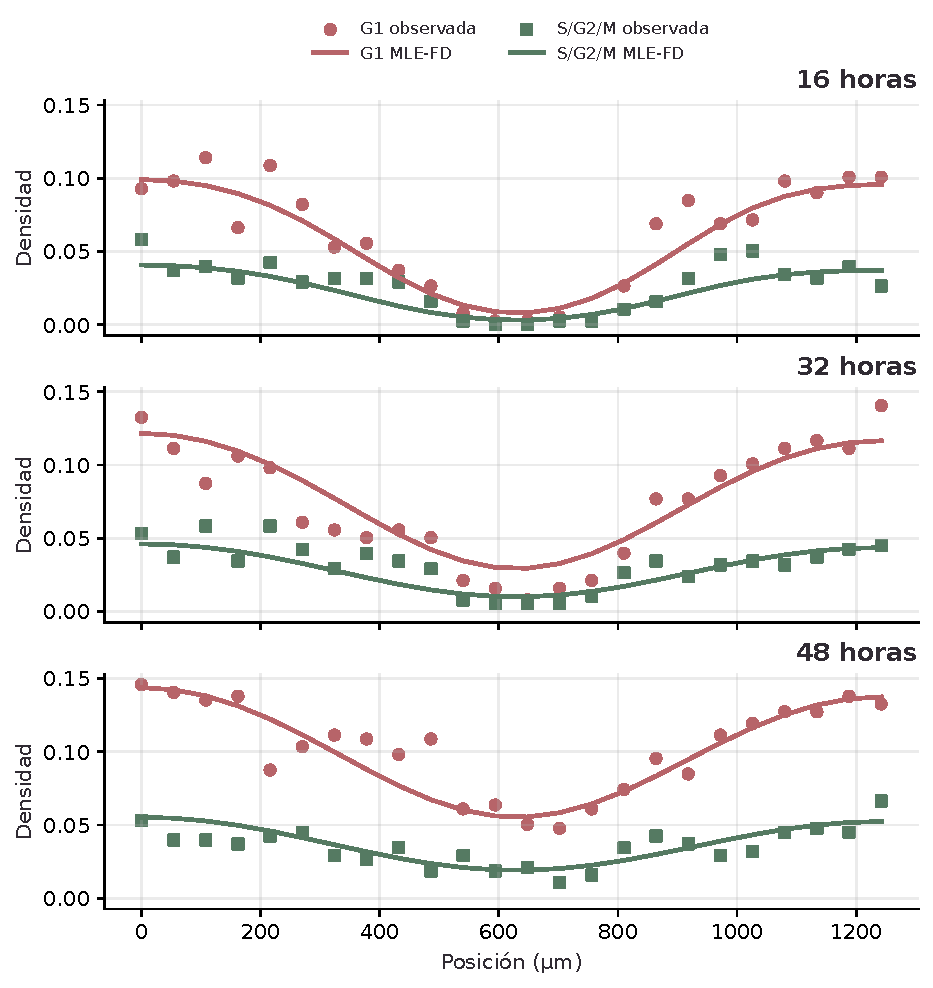
\includegraphics[width=.85\textwidth]{figuras/ajuste.pdf}
\caption{Redibujo del ajuste clásico a los tres tiempos posteriores al inicial, a partir de las tablas de residuos del escenario 1. Son datos de ajuste, no un conjunto de prueba independiente.}
\end{figure}

\section{Intervalos de las tablas de respaldo}
\begin{center}\small
\begin{tabular}{llrrr}\toprule
Escenario & Parámetro & MLE & Inferior & Superior\\\midrule
1 & $D$ &709.8526&365.0697&1207.6765\\
1 & $k_r$ &0.028882&0.018056&0.039907\\
1 & $k_g$ &0.071624&0.054861&0.091171\\
2 & $D_r$ &601.8408&\multicolumn{2}{c}{Sin cruce en $[1,2000]$}\\
2 & $D_g$ &919.1594&\multicolumn{2}{c}{Sin cruce en $[1,2000]$}\\
2 & $k_r$ &0.029142&0.017628&0.040792\\
2 & $k_g$ &0.071336&0.054560&0.092419\\\bottomrule
\end{tabular}
\end{center}
El póster destaca el intervalo de $D$. La tabla completa permite responder si las tasas también se debilitan: sus intervalos siguen delimitados en ambos escenarios, mientras las difusiones separadas son especialmente problemáticas.

En el escenario 1 la anchura relativa $(U-L)/\widehat\theta$ es aproximadamente $1.187$ para $D$, $0.757$ para $k_r$ y $0.507$ para $k_g$. Según esta medida, $D$ tiene la mayor incertidumbre relativa de los tres. Esto no requiere comparar unidades incompatibles ni decir que los otros parámetros se conocen con exactitud.

\begin{figure}[htbp]\centering
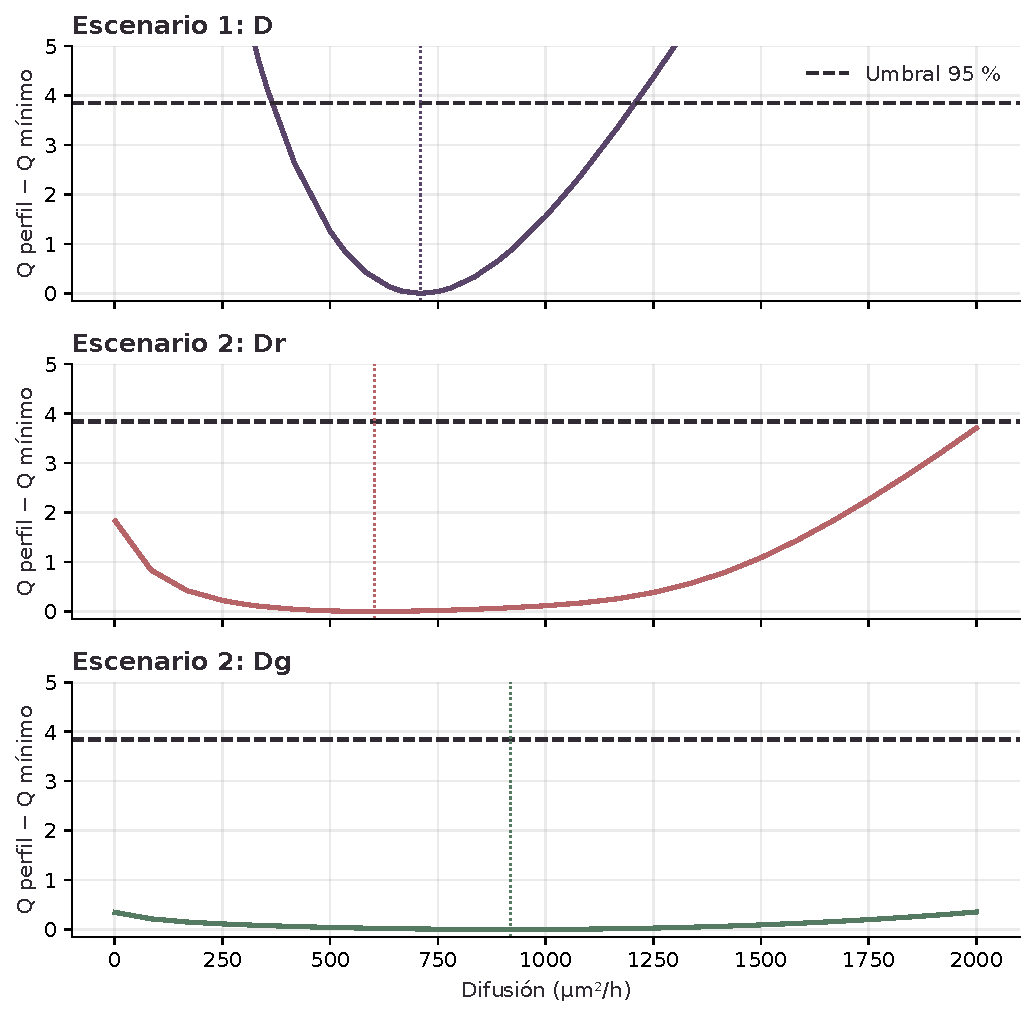
\includegraphics[width=.82\textwidth]{figuras/perfiles.pdf}
\caption{Perfiles redibujados en una escala vertical común cercana al umbral. El póster final usa paneles con distintas escalas verticales; al explicarlos debe compararse el cruce con el umbral, no únicamente su apariencia visual.}
\end{figure}

\section{Estabilidad estrecha e intervalo ancho no se contradicen}
La DE PINN de $D$ es $3.04$, pero el IC perfilado va aproximadamente de $365$ a $1208$. Las semillas mantienen las observaciones fijas y cambian el procedimiento de optimización. El perfil pregunta cuánto pueden variar los parámetros sin deteriorar demasiado la verosimilitud de esos datos bajo el ruido supuesto.

No se debe construir un supuesto IC para el parámetro como $700.09\pm1.96(3.04)$ ni como $700.09\pm t\,3.04/\sqrt{10}$. Tales operaciones describirían, con supuestos adicionales, propiedades de la distribución de resultados del algoritmo o de su media condicional a los datos, no la incertidumbre experimental del parámetro físico.

\begin{figure}[htbp]\centering
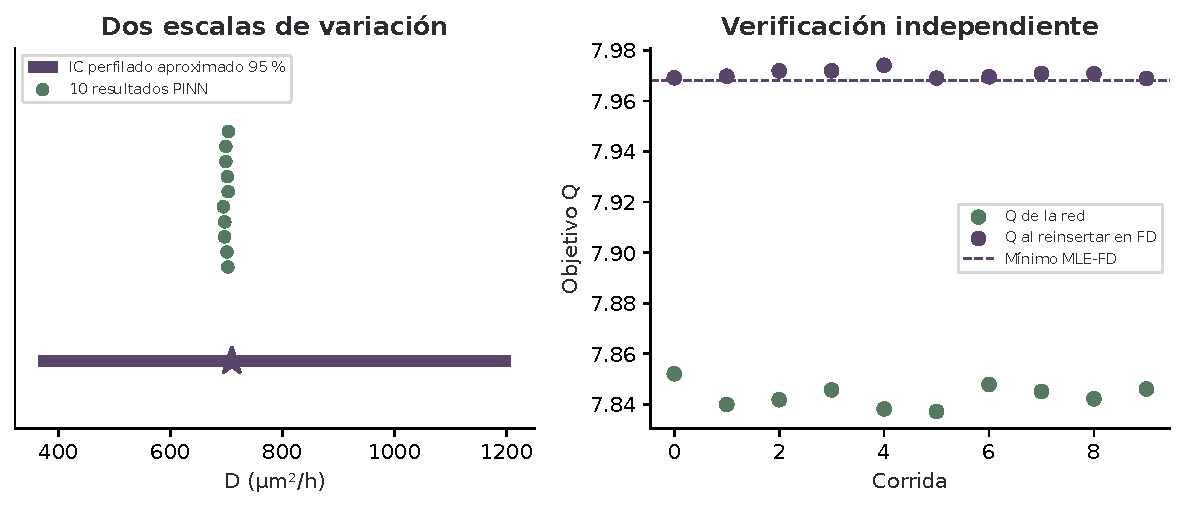
\includegraphics[width=\textwidth]{figuras/estabilidad_verificacion.pdf}
\caption{Izquierda: escala de la dispersión de diez estimaciones frente al IC perfilado. Derecha: objetivo evaluado en la red y objetivo al resolver FD con sus parámetros. Diagnósticos de respaldo para estudiar la interpretación del póster.}
\end{figure}

\section{Por qué verificar la PINN con otro solucionador}
La red puede ajustar los datos sin satisfacer exactamente la EDP. Por eso se toma $\widehat\theta_{\rm PINN}$, se resuelve nuevamente el sistema con FD y se evalúa ese campo en las observaciones:
\[
Q_{\rm FD}(\widehat\theta_{\rm PINN})
\quad\hbox{frente a}\quad Q_{\rm red}(w,\widehat\theta_{\rm PINN}).
\]
En el escenario 1, los objetivos de la red son aproximadamente $7.837$--$7.852$, menores que el mínimo clásico $7.968$. Tras reinserción, son aproximadamente $7.969$--$7.974$: ya no mejoran el mínimo clásico. El RMSE recalculado está entre $0.011762$ y $0.011766$, frente a $0.011762$ del MLE.

Esto no demuestra superioridad predictiva de la red. Muestra por qué era necesario evaluar los parámetros a través de una solución dinámica independiente de la aproximación neuronal. La diferencia entre ambos objetivos es compatible con el margen de incumplimiento de la EDP y con diferencias numéricas; no atribuye toda la discrepancia a una causa única.

La independencia aquí es computacional, no experimental. FD usa los mismos datos, ecuaciones y condición inicial; esta verificación no valida biológicamente el modelo ni constituye una prueba fuera de muestra.

\section{Escenario 2: dispersión de las difusiones}
\begin{figure}[htbp]\centering
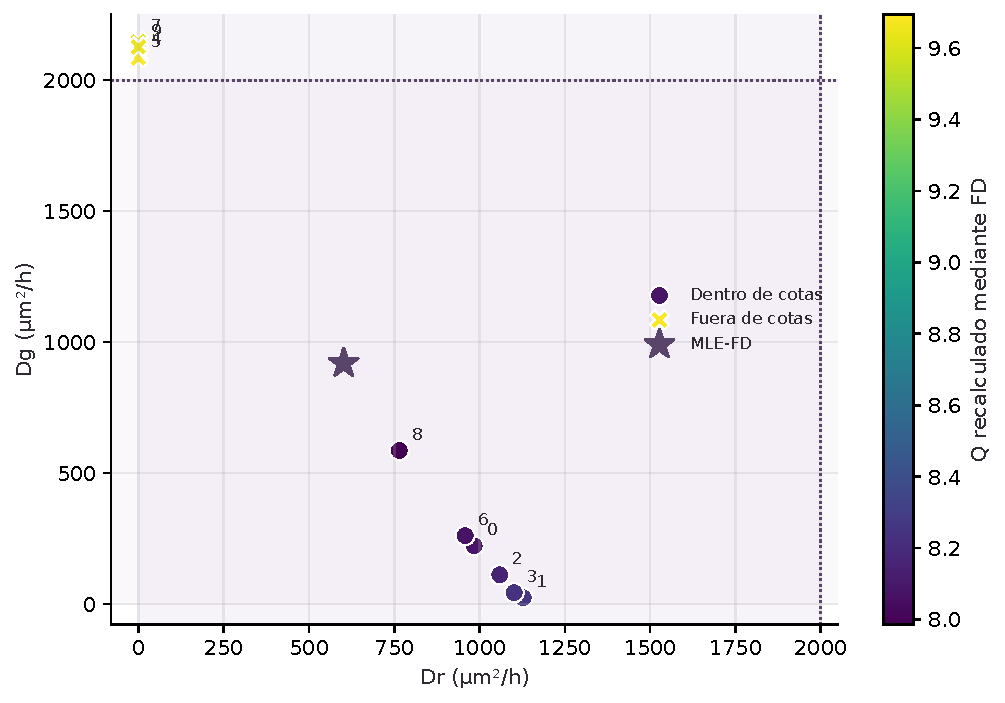
\includegraphics[width=.9\textwidth]{figuras/dispersion.pdf}
\caption{Diez resultados PINN del escenario 2. Color: objetivo recalculado con FD. Las cruces señalan los cuatro resultados fuera de las cotas clásicas; los números identifican corridas. El póster final muestra estos resultados en una figura más compacta.}
\end{figure}
Los puntos muestran combinaciones muy diferentes de $D_r,D_g$. Cuatro tienen $D_r<1$ y $D_g>2000$; la positividad de la parametrización neuronal no evita esos resultados. Las cotas clásicas y neuronales no definen el mismo espacio factible.

Los RMSE FD del escenario 2 van aproximadamente de $0.011774$ a $0.012973$. Ajustes de magnitud semejante pueden acompañar parámetros muy distintos. Sin embargo, todos los puntos no son óptimos equivalentes: los colores y los objetivos muestran diferencias. La dispersión mezcla geometría poco informativa, optimización, aproximación y restricciones distintas. Los perfiles clásicos aportan evidencia independiente de debilidad práctica; la nube por sí sola no demostraría su causa.

\section{Cuánto mejora el ajuste al añadir una difusión}
Las tablas dan
\[
Q_1=7.96797547,\quad Q_2=7.95705053,\quad Q_1-Q_2=0.01092494.
\]
La reducción relativa es aproximadamente $0.137\%$. Añadir un parámetro no debería empeorar el óptimo global porque el modelo simple está contenido en el ampliado. Una pequeña mejora es esperable por flexibilidad; no basta para justificar mayor complejidad.

Como respaldo adicional, con $\sigma$ fija y el mismo conjunto de datos, $\mathrm{AIC}=Q+2p+\text{constante}$. Las tablas registran $13.968$ y $15.957$ sin constante común: diferencia cercana a $1.99$ a favor del escenario 1. Es una preferencia modesta y condicional; no una prueba de que $D_r=D_g$ sea una verdad biológica.

El contraste de modelos anidados podría relacionar $Q_1-Q_2$ con un estadístico de razón de verosimilitudes bajo condiciones regulares. En un problema débilmente identificado conviene no convertir esa aproximación en una conclusión más fuerte que la evidencia disponible. El póster se centra en la mejora mínima y los perfiles.

\section{Sensibilidad al estado inicial}
Con interpolación inicial en lugar de cosenos, las tablas de verificación dan $D\approx696.21$, $k_r\approx0.02914$ y $k_g\approx0.07238$. Frente al análisis principal, los cambios son aproximadamente $-1.92\%$, $+0.89\%$ y $+1.05\%$. En el escenario 2, $D_g$ cambia cerca de $-4.23\%$.

Es una comparación de sensibilidad existente, no un intervalo de confianza ni una propagación completa del error inicial. Explica por qué no deben mezclarse sin más estimaciones de distintas versiones, incluido el ajuste clásico anterior con $D\approx733.48$. Cambiar la preparación y formulación cambia el problema efectivamente resuelto.

\chapter{Diagnóstico, limitaciones y extensiones}
\section{Diagnóstico de residuos}
Un residuo es $e=y-\widehat y$. Conviene examinarlo por población, posición, tiempo y valor ajustado. Patrones de signo consecutivos en el espacio sugieren revisar correlación, discretización o forma del modelo; dispersión creciente con densidad sugiere heterocedasticidad. Un patrón no identifica por sí solo cuál causa lo produjo.

\begin{figure}[htbp]\centering
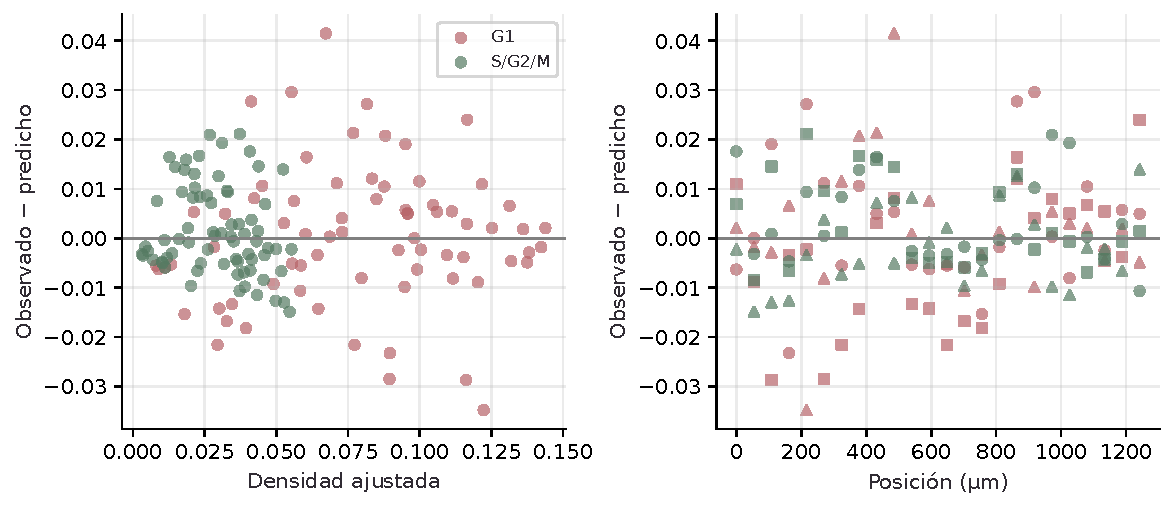
\includegraphics[width=\textwidth]{figuras/residuos.pdf}
\caption{Residuos del ajuste compartido, reconstruidos desde las tablas. Son una ayuda de diagnóstico; no constituyen por sí solos una validación de independencia, normalidad u homocedasticidad.}
\end{figure}
Una prueba de normalidad que no rechace no demuestra normalidad. Tampoco una media residual cercana a cero descarta correlación. En observaciones de un mismo cultivo, la estructura espacial y temporal debe considerarse en cualquier interpretación probabilística fuerte.

\section{Implicaciones de la escala de ruido}
El RMSE observado es alrededor de $0.01176$, bastante menor que $0.05$. La estimación descriptiva $\sqrt{\mathrm{SSE}/(144-3)}$ sería aproximadamente $0.01189$. Esta diferencia motiva sensibilidad al supuesto de ruido. No autoriza a reemplazarlo silenciosamente después de mirar los resultados ni a presentar intervalos nuevos sin recalcularlos.

Si $\sigma$ se estimara junto con $\theta$, su MLE gaussiano sería $\widehat\sigma^2(\theta)=\mathrm{SSE}(\theta)/n$. Al perfilarla, la razón de verosimilitudes para $\theta$ involucraría
\[
n\log\frac{\mathrm{SSE}_p(\psi)}{\mathrm{SSE}(\widehat\theta)},
\]
en lugar de una diferencia de SSE dividida por una $\sigma^2$ conocida. Esa es una extensión del análisis, no la fórmula utilizada para los intervalos del póster.

\section{Alcance de la evidencia}
\begin{longtable}{p{.46\textwidth}p{.46\textwidth}}
\toprule Afirmación defendible & Afirmación excesiva\\\midrule
La PINN final concuerda con MLE-FD en el escenario 1. & La PINN recuperó los parámetros verdaderos del cultivo.\\
El IC de $D$ es delimitado y amplio. & $D$ está determinado con alta precisión.\\
Los perfiles separados no cruzan en las cotas exploradas. & Se demostró no identificabilidad estructural.\\
Las semillas finales presentan poca dispersión con difusión común. & La incertidumbre estadística es la DE de diez semillas.\\
La EDP aporta una restricción al aprendizaje. & Más colocación equivale a más datos experimentales.\\
La reinserción FD apoya la coherencia de los parámetros. & Se validó la capacidad de generalización biológica.\\
El modelo ampliado mejora muy poco el ajuste. & Se demostró que las dos difusiones reales son iguales.\\\bottomrule
\end{longtable}

\section{Cómo sería un estudio de cobertura}
\begin{enumerate}
\item Elegir un parámetro generador conocido y resolver la EDP con precisión suficiente.
\item Generar muchos conjuntos de observaciones con un mecanismo de ruido especificado.
\item Reajustar cada conjunto con el procedimiento completo, incluidos reinicios y fallos.
\item Construir intervalos en cada réplica y registrar cuántos contienen el valor generador.
\item Estimar cobertura, sesgo, RMSE paramétrico, anchura y tasa de fallos; cuantificar error Monte Carlo.
\end{enumerate}
Si $B$ réplicas producen cobertura empírica $\widehat c$, su error estándar Monte Carlo es aproximadamente $\sqrt{\widehat c(1-\widehat c)/B}$. Cincuenta réplicas, por ejemplo, darían un error aproximado de $0.031$ alrededor de $0.95$: distinguir diferencias pequeñas requiere más simulaciones. Este cálculo es didáctico; no describe un experimento de cobertura realizado para el póster.

\section{Bootstrap, Bayes y diseño de observaciones}
Un bootstrap paramétrico simularía datos desde el modelo ajustado y repetiría la inferencia. Un remuestreo ingenuo de filas podría destruir la estructura espacial y temporal. El esquema debe respetar la unidad experimental y el modelo de dependencia. Diez semillas con los mismos datos no son bootstrap.

Una extensión bayesiana especificaría $p(\theta)$ y usaría $p(\theta\mid y)\propto L(y\mid\theta)p(\theta)$. Una B-PINN podría incluir pesos y parámetros en una distribución posterior; necesita una formulación probabilística y un método de inferencia. No basta llamar bayesiana a una red determinista con varias semillas. En direcciones poco informadas, el prior puede influir mucho: una posterior estrecha no demuestra que los datos aportaron toda esa precisión.

El diseño experimental buscaría mediciones que separen las sensibilidades de $D_r$ y $D_g$: otros tiempos, regiones con gradientes informativos o réplicas biológicas. Una estrategia local podría maximizar el menor autovalor de Fisher o su determinante. Es una propuesta futura; el proyecto no ha establecido qué diseño es óptimo ni que cualquier aumento de datos resuelva el problema.


\chapter{Conclusiones}
La simplificación de una difusividad compartida permite delimitar un intervalo perfilado para $D$, aunque su amplitud revela incertidumbre considerable. La incorporación de una segunda difusividad introduce una dirección de compensación que los datos disponibles restringen débilmente. Una mejora mínima del ajuste no compensa automáticamente la pérdida de precisión paramétrica.

Las PINNs proporcionan estimaciones finales próximas al MLE en el escenario compartido. La estabilidad depende del procedimiento de entrenamiento y reinicio. Al separar difusiones, la dispersión aumenta; ese comportamiento es compatible con la debilidad de los perfiles, pero no constituye por sí mismo una medida de incertidumbre estadística.

Los intervalos se interpretan condicionalmente al modelo gaussiano independiente, $\sigma=0.05$, la condición inicial fijada, el dominio, las cotas y el solucionador numérico. Las extensiones prioritarias son estudiar convergencia de malla, propagar incertidumbre del estado inicial, evaluar sensibilidad al ruido y realizar simulaciones de recuperación y cobertura antes de afirmar garantías inferenciales más amplias.

\chapter{Reproducibilidad y procedencia}
\section{Evidencia conservada}
El repositorio incluye el póster presentado en \texttt{docs/Poster\_PINNs\_FUCCI.pdf}; las tablas de máxima verosimilitud, perfiles, Fisher, residuos, sensibilidad y entrenamientos se conservan en \texttt{results/published/}. Los datos reorganizados se distribuyen como CSV numérico en \texttt{data/}, con la estructura de observaciones y la normalización originales. El registro \texttt{docs/PROCEDENCIA.md} describe selección y transformaciones.

\section{Código y notebooks}
\texttt{src/common.py} implementa la carga de datos, el suavizado coseno y el solucionador de diferencias finitas. \texttt{src/fit\_fd.py} ajusta los dos escenarios; \texttt{src/pinn.py} implementa la PINN; \texttt{src/run\_study.py} controla réplicas y reinicios. Los notebooks de verificación (01) y de perfiles e intervalos (02), disponibles en \texttt{notebooks/}, reutilizan el mismo solucionador y guardan nuevos resultados en \texttt{results/generated/}.

\section{Niveles de reproducción}
La reconstrucción de tablas y figuras desde resultados publicados no requiere entrenar una red. El recálculo MLE y de perfiles sí integra repetidamente la EDP y puede consumir tiempo. El reentrenamiento de PINNs requiere PyTorch y un presupuesto mayor; las diez réplicas originales no se han repetido para esta edición documental. No se incluyen todos los pesos entrenados ni registros completos de cada ejecución, de modo que no se garantiza reconstrucción bit a bit de los campos neuronales originales.

Los valores por defecto del código no certifican todos los hiperparámetros efectivos de las corridas archivadas. Las tablas contienen evidencia de los parámetros finales y métricas guardadas; las nuevas corridas deben conservar configuración, semillas, versiones y salidas propias. El estudio sintético disponible en el controlador es una herramienta para trabajo posterior, no evidencia de cobertura ya validada en este informe.

\section{Selección editorial y atribución}
Se conserva una sola línea numérica, correspondiente al dominio $[0,1242]$, 139 nodos y condición inicial coseno de grado 8. El ajuste anterior con dominio extendido e inicial interpolada pertenece a los antecedentes y se excluye para no mezclar cifras. También se omiten conversaciones, guiones de exposición, ejercicios de estudio, paquetes de contexto, versiones anteriores y auxiliares de compilación.

El modelo y los datos proceden de Simpson y colaboradores. La implementación neuronal y sus experimentos corresponden al trabajo de Sergio Alejandro Villada Arias; la inferencia y el análisis estadístico fueron desarrollados por Bamsi Mendez Posada en el marco del proyecto conjunto. La reorganización del repositorio y la adaptación editorial de este informe contaron con asistencia de IA. No se redistribuyen los artículos científicos completos ni se establece una licencia global que sustituya las condiciones de materiales ajenos.

\section{Compilación del documento}
Desde \texttt{docs/}, compilar \texttt{Informe\_PINNs\_FUCCI.tex} dos veces con pdfLaTeX, o ejecutar \texttt{latexmk -pdf Informe\_PINNs\_FUCCI.tex}. Se requiere una distribución LaTeX con los paquetes declarados en el preámbulo. Las figuras PDF están incluidas; no es necesario reentrenar modelos para compilar el informe.
\begin{thebibliography}{9}
\addcontentsline{toc}{chapter}{Referencias}
\bibitem{simpson} Simpson, M. J., Baker, R. E., Vittadello, S. T. y Maclaren, O. J. (2020). Practical parameter identifiability for spatio-temporal models of cell invasion. \emph{Journal of the Royal Society Interface}, 17, 20200055. \url{https://doi.org/10.1098/rsif.2020.0055}. Fuente del problema biológico y del modelo; distinguir sus resultados de las estimaciones propias.
\bibitem{raissi} Raissi, M., Perdikaris, P. y Karniadakis, G. E. (2019). Physics-informed neural networks: A deep learning framework for solving forward and inverse problems involving nonlinear partial differential equations. \emph{Journal of Computational Physics}, 378, 686--707. \url{https://doi.org/10.1016/j.jcp.2018.10.045}. Referencia metodológica de PINNs; la arquitectura concreta de este informe procede del código del proyecto.
\bibitem{raue} Raue, A., Kreutz, C., Maiwald, T., Bachmann, J., Schilling, M., Klingmüller, U. y Timmer, J. (2009). Structural and practical identifiability analysis of partially observed dynamical models by exploiting the profile likelihood. \emph{Bioinformatics}, 25(15), 1923--1929. \url{https://doi.org/10.1093/bioinformatics/btp358}. Referencia del enfoque de perfiles citado en el póster.
\bibitem{datos} Simpson y colaboradores (2020). Material suplementario de Practical parameter identifiability for spatio-temporal models of cell invasion. \url{https://doi.org/10.6084/m9.figshare.c.4862265.v1}. En el proyecto se conservan una transcripción CSV del Excel reorganizado.
\end{thebibliography}
\end{document}
